\section{Systementwurf}
\textcolor{red}{Lorem ipsum dolor sit amet, consetetur sadipscing elitr, sed diam nonumy eirmod tempor invidunt ut labore et dolore magna aliquyam erat, sed diam voluptua. Lorem ipsum dolor sit amet, consetetur sadipscing elitr, sed diam nonumy eirmod tempor invidunt ut labore et dolore magna aliquyam erat, sed diam voluptua. Lorem ipsum dolor sit amet, consetetur sadipscing elitr, sed diam nonumy eirmod tempor invidunt ut labore et dolore magna aliquyam erat, sed diam voluptua. Lorem ipsum dolor sit amet, consetetur sadipscing elitr, sed diam nonumy eirmod tempor invidunt ut labore et dolore magna aliquyam erat, sed diam voluptua.}

\subsection{Vorgehensweise Anforderungserhebung}
Die Anforderungen für ein zu konzipierende System wurden vor dem Hintergrund der Evaluation des Geschäftsprozesses erhoben. Außerdem wurde bei der Erfassung der Anforderung darauf geachtet, das der Prototyp beim Praxispartner als Unterstützung für zukünftige Innovationsfragen herangezogen werden kann. Wie von \citet{Dick2017, HullElizabeth2011} beschrieben, kann das Prototyping selbst bereits als Anforderungsanalyse angesehen werden, jedoch wurde für die prototypische Implementierung des Systementwurfs eine gesonderte Anforderungsanalyse durchgeführt. Ziel dieser Vorgehensweise ist eine präzise Definition und Eingrenzung der Anforderungsbeschreibung während des Konzeptions- und Implementierungsprozesses.

Im Zuge der Anforderungserhebung wurden die Anforderungen in Zusammenarbeit mit dem Praxispartner entwickelt. Die Anforderungen wurden dabei in textueller Form nach einem festen Muster in Anlehnung an \citet{PohlKlaus2015} definiert. Ergänzt wurden die textuellen Anforderungen um Prozessdiagramme und Mockups der Nutzeroberflächen. Der Fokus des konzipierten System liegt dabei allerdings auf eigentlichen Blockchain Netzwerk und weniger auf der Benutzungsoberfläche.

Die Anforderungen wurden untergliedert in funktionale Anforderungen, Rahmenbedingungen und Qualitätsanforderungen. Ebenso wurden die Anforderungen hierarchisch strukturiert und um eine Quelle ergänzt nach \citet{Koelsch2016}. Dies soll die Nachverfolgbarkeit der Anforderungen während der Evaluation unterstützen.

\subsection{Das Ziel: Chargenrückverfolgung innerhalb der Fleischwarenindustrie} \label{goal-description}
Das System soll unter experimentellen, abstrahierten Bedingungen die Chargenrückverfolgung von Schweinen innerhalb der Produktions- und Wertschöpfungskette realisieren. Dafür muss das System den Prozess vom Erzeuger bis zum Groß- und Einzelhandel unterstützen. Konkret sollen Erzeuger neue Tiere im Blockchain Netzwerk registrieren und einer Charge zuordnen können. Bereits registrierte Tiere sollen zur Weiterverarbeitung freigegeben werden können und ein Eigentumswechsel muss durch das System abbildbar sein. Die Gesamtheit der Transaktionen zwischen den Teilnehmern der Wertschöpfungskette kann als Graph angesehen werden. Anhand dieses Graphen soll eine Rückverfolgbarkeit einer Charge gewährleistet werden. Über eine Benutzungsoberfläche sollen die Teilnehmer jederzeit in der Lage sein den Graphen einsehen zu können. Für die technische Umsetzung des System spielt die Benutzungsoberfläche jedoch eine nachgelagerte Priorität. Hauptaugenmerk des Systementwurfs liegt auf dem technologischen Aufbau des Blockchain Netzwerk und den Schnittstellen für etwaige Drittsysteme zur automatischen Erfassung von Tieren. Eine automatische Erfassung von neuen Tieren kann beispielsweise über \ac{iot}-Sensoren in Schlachthaken erfolgen. Ebenso würde sich ein Eigentumswechsel, wenn Tiere vom Erzeuger an den Schlachthof verkauft werden, über \acs{rfid}-Chips und entsprechende Lesegeräte, welche per Schnittstelle mit dem Blockchain Netzwerk verbunden sind, abwickeln lassen \citep{Dorri2017, Samaniego2016}.

\subsection{Die Wertschöpfungskette im Detail}
Nachfolgend soll eine kurze Erläuterung der in Kapitel \ref{goal-description} erwähnten Wertschöpfungskette dazu dienen, die Daten- und Warenströme zwischen den Teilnehmern klar zu trennen und die für diesen Systementwurf wichtigen Informationen herauszuarbeiten. Da eine Chargenrückverfolgung nur gewährleistet werden kann, wenn in den vorgelagerten Prozessen die nötigen Informationen in einem System bereitgestellt wurden, soll auf die Teilschritte vom Erzeuger zum Endverbraucher eingegangen werden.

Die Fleischwirtschaft hat in den letzten Jahren einen Strukturwandel vollzogen, welcher auch Auswirkungen auf die eigentliche Tätigkeit sowie die Lieferanten- und Abnehmerbeziehungen zwischen den Unternehmen hat \citep{Nolte2006}. Als eine der zentralen Ursachen für den Strukturwandel wird die Konzentrierung der Schlachtunternehmen gezählt. Inzwischen werden deutlich mehr als 50\% aller Schweine in Deutschland von drei Unternehmen geschlachtet - Tönnies, Vion und Westfleisch. Unter Beachtung anderer Wirtschaftszweige wie beispielsweise der Geflügelschlachtung, die noch wesentlich stärker konzentriert ist, und dem Hintergrund das in Ländern wie Dänemark die Schlachtung nur noch von zwei Unternehmen durchgeführt wird, wird deutlich das der Konzentrationsprozess in Deutschland auf der Schlachtstufe noch nicht abgeschlossen ist. Im Gegensatz dazu ist der Viehandel und die Landwirtschaft weniger stark konzentriert, weshalb sie sich in einer schwachen Verhandlungsposition befinden. Um dieser schwachen Verhandlungsposition entgegenzuwirken sind Unternehmen des Viehandels dazu gezwungen immer größere Mengen an Schlachttieren zu einer Charge zu bündeln. Ebenfalls sind zahlreiche unternehmensübergreifende Kooperationen im Viehandel zu beobachten \citep{Voss2010}.

Vom Erzeuger bis zum Endverbraucher ist die Wertschöpfungskette in Deutschland sehr vielfältig ausgeprägt \citep{Freund1997}. Der Hauptabsatzweg für Schweinemäster läuft entweder über eine direkt Vermarktung an Schlachtbetriebe (einstufige Vermarktung) oder indirekt über den privaten Viehandel, Viehvermarktungsgenossenschaften oder Erzeugergemeinschaften (zweistufige Vermarktung). Die Schlachtstufe lässt sich daher als Flaschenhals der Wertschöpfungskette aus Sicht der Schweinemäster betrachten. Um klar bestimmen zu können welche Informationen und virtuellen Assets in dem Blockchain Netzwerk abgebildet werden müssen, werden der Waren- und Datenstrom nachfolgend einzeln betrachtet.

\subsubsection{Betrachtung des Warenstroms}

Die Wertschöpfungskette vom Erzeuger bis zum Fleischwarenproduzenten gliedert sich grob in vier Produktionsschritte, welche nachfolgend kurz beschrieben und in Abbildung \ref{fig:structure-value-chain-meat-industry-numbered} schematisch dargestellt werden. Dabei sind sieben Parteien direkt in den Gesamtprozess bis zum Verbraucher involviert und eine achte Partei wirkt indirekt als Vermittler zwischen den anderen Parteien mit.

\begin{landscape}
    \begin{figure}
        \centering
        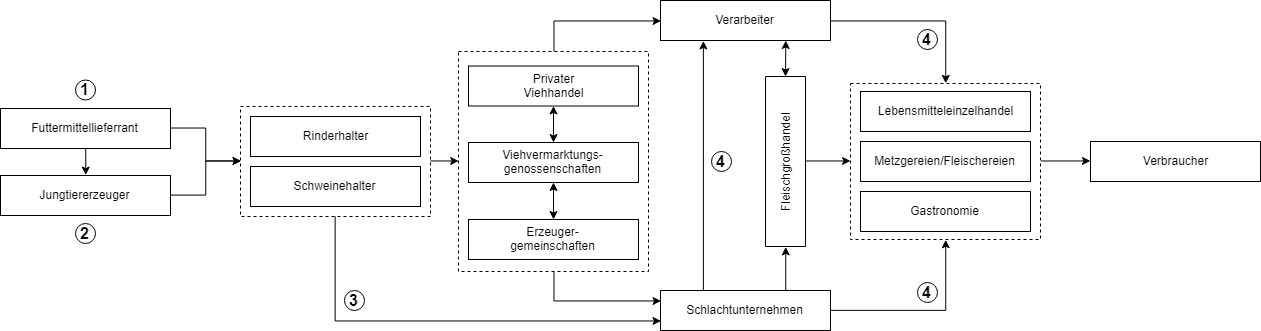
\includegraphics[width=1.0\linewidth]{pictures/structure-value-chain-meat-industry-numbered}
        \caption[Struktur der Wertschöpfungskette der Fleischwirtschaft]{Struktur der Wertschöpfungskette der Fleischwirtschaft nach \citet{Petersen2010, Voss2010, Beck2008}}
        \label{fig:structure-value-chain-meat-industry-numbered}
    \end{figure}
\end{landscape}

\noindent
Der Warenstrom beginnt mit (1) der Futtermittellieferung an die Jungtiererzeuger und Viehhalter. Jeder Betrieb wird dabei über die \ac{iln} global eindeutig identifiziert. (2) Nach der Aufzucht der Jungtiere werden diese durch Transportunternehmen zu den Viehhaltern transportiert. In den Mästbetrieben bleiben die Tiere dann bis zur Schlachtreife. (3) Im Auftrag der Schlacht- und Zerlegebetriebe werden die schlachtreifen Tiere von den Mästbetrieben angeliefert. Nach der Verarbeitung der Tiere in den Schlacht- und Zerlegebetrieben werden diese (4) an die verschiedenen Abnehmer geliefert, um letztendlich zu Produkten für den Verbraucher weiterverarbeitet zu werden. Hieraus ergibt sich, dass mindestens an den erwähnten vier Punkten der Wertschöpfungskette eine Prozessschnittstelle vom Blockchain Netzwerk bedient werden können muss.

\subsubsection{Informationswege in der Fleischindustrie}

Abbildung \ref{fig:data-stream-meat-industry} zeigt den nachfolgend beschriebenen Datenstrom zwischen den einzelnen Produktionsstufen der Fleischindustrie. \textcolor{red}{Referenz zu Anforderungen} (1) Jungtiererzeuger und Viehhalter senden jeweils eine Futtermittelbestellung an den Futtermittellieferanten. (2) Nach erfolgreicher Lieferung informiert der Futtermittellieferant den privaten Viehhandel bzw. die Viehvermarktungsgenossenschaften respektive Erzeugergemeinschaften. Die Viehhalter melden einerseits (3) die Aufnahme der Jungtiere und andererseits (4) die schlachtreife von Tieren an die Viehvermarktungsgenossenschaften zur Weitervermittlung and die Schlacht- und Zerlegebetriebe. (5) Bei der Weitervermittlung werden die Informationen über die Tiere an Schlacht- und Zerlegebetriebe übermittelt. (6) Mit dem Lieferauftrag initiiert das Schlachtunternehmen die Bestellung und den Transport der schlachtreifen Tiere. (7) Die Viehvermarktungsgenossenschaften bestätigen den Lieferauftrag mit einer elektronischen Ankündigung der Schlachtviehlieferung. Bei der Anlieferung der Tiere gleicht das Schlachtunternehmen die tatsächliche angelieferte Anzahl mit der bestellten Menge ab und meldet die Werte an die Viehvermarktungsgenossenschaften zurück. Mit dieser Wareneingangsmeldung kann die Viehvermarktungsgenossenschaft den Bestand und die aktuellen Standorte der Tiere aktualisieren. (9) Im Schlachtunternehmen werden dann weitere Informationen zu den Stammdaten der Tiere erfasst. Dazu zählen die \ac{vvvo}-Nummern der Landwirte, eine Vergabe Partie-Nummer je Lkw und eine fortlaufende Schlachtnummer. (10)Anschließend werden die Informationen wieder an die Viehvermarktungsgenossenschaft zurück gemeldet. (11) Letztendlich bedienen die Schlacht- und Zerlegebetriebe die Bestellungen der Fleischwerke, Lebensmitteleinzelhandel, Metzgereien und die Gastronomie. (12) Hier werden dann auch die letzten Stammdaten zu den Produkten erfasst und verknüpft wie beispielsweise Artikelbezeichnung, Stückzahl, Schlachtdatum und Schlacht-Nummer. (13) Mit der Zuordnung der zuverarbeitenden Fleischerzeugnisse zum Lieferschein in einem \ac{erp}-System enden die betrachteten Informationswege in der Fleischindustrie.

\begin{figure}[H]
	\centering
	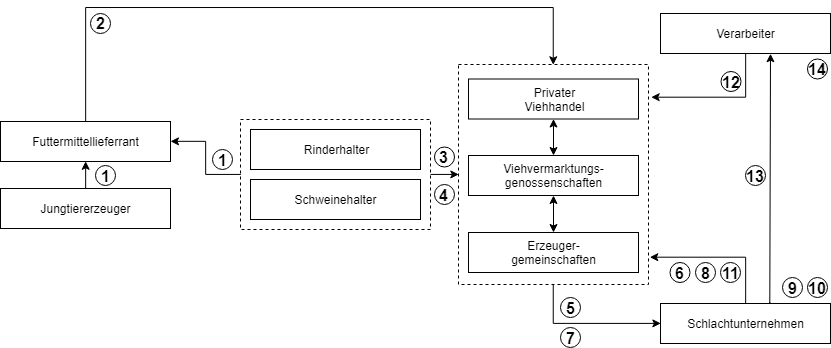
\includegraphics[width=1\linewidth]{pictures/data-stream-meat-industry-numbered}
	\caption[Datenströme innerhalb der Wertschöpfungskette]{Datenströme innerhalb der Wertschöpfungskette \textcolor{red}{QUELLE}}
	\label{fig:data-stream-meat-industry}
\end{figure}

%1 Futtermittelbestellung\\
%2 Meldung über Futtermittellieferung (DESADV optional)\\
%3 Aufnahmemeldung der Jungtiere\\
%4 Meldung schlachtreifer Schweine\\
%5 Weitervermittlung schlachtreifer Schweine an Schlachthof\\
%6 Lieferauftrag\\
%7 elektronische Ankündigung der Schlachtviehlieferung\\
%8 Wareneingangsmeldung (optional)\\
%9 Erfassung VVVO Landwirt, Vergabe Partie-Nr. je Lkw (je vom Schlachthof); Aufbringen einer fortlaufenden Schlacht-Nr. (manuell)\\
%10 Meldung Schlachtdaten\\
%11 Bestellung Schweinehälften\\
%12 u.a. Artikelbezeichnung, Stückzahl, Schlachtdatum, Schlacht-Nr., Schadenskennzeichen\\
%13 Automatische Zubuchung Schweinehälfte und Gewicht, Automatische Verknüpfung mit Lieferschein im ERP-System

\subsection{Geschäftsprozess Chargenrückverfolgung}
Die vorrangegangene Betrachtung der Waren- und Datenströme macht deutlich an welchen Schnittpunkten der Wertschöpfungskette Informationen gesammelt und zentral über die Viehvermarktungsgenossenschaften verwaltet werden. Dies ist wichtig für den Geschäftsprozess der Chargenrückverfolgung, da eine lückenlose Rückverfolgbarkeit nur dann gewährleistet ist wenn vom Erzeuger bis zum Endverbraucher alle Informationen konsistent und transparent zur Verfügung stehen. Dabei spielt es keine Rolle von welcher Seite der Wertschöpfungskette eine Rückverfolgung durchgeführt wird im Sinne des Down- und Uptracing.

Der Vergleich zwischen dem Prozess der Rückverfolgung wie er aktuell durchgeführt wird (Ist-Prozess) und wie er mit dem Einsatz eines Blockchain Systems aussehen kann (Soll-Prozess) dient dazu die funktionalen Anforderungen ableiten zu können.

\paragraph{Ist-Prozess}
Der Ist-Prozess durchläuft die Schritte von der Verbrauchermeldung bis zur Information der anderen Teilnehmer in der Wertschöpfungskette. Dabei wird anhand der Produktkennung und Verbrauchermeldung ermittelt zu welcher Produktcharge die Meldung gehört. Hierfür wird eine vielzahl an Software und Datenbeständen benötigt. Dazu zählt die Office Suite von Microsoft und ein ERP-System in Kombination mit einer Lieferantenmanagement- (SAP SRM) und Vertriebslösung (SAP CRM). Nach der Zuordnung der Verbrauchermeldung zur Produktcharge wird im Sinne des Uptracing die Charge bis zum Erzeuger zurückverfolgt, um zu prüfen in welchem Produktionsschritt das gemeldete Problem entstanden ist. Hierdurch können Maßnahmen zum Abstellen des Problem erarbeitet werden, die an alle Teilnehmer übermittelt werden. Die Chargeninformationen werden bereitsgestellt von einer zentralen Instanz, der Viehvermarktungsgenossenschaft. Dies bedeutet, liegen der Viehvermarktungsgenossenschaft lückenhafte bzw. manipulierte Datensätze vor besteht die Gefahr eine Rückverfolgung nicht vollständig durchführen zu können. Ebenfalls muss der Verbraucher der Viehvermarktungsgenossenschaft vertrauen für vollständig- und korrektheit der bereitgestellten Informationen. Nachdem alle Teilnehmer informiert sind ist der Prozess der Rückverfolgung abgeschlossen. Entsprechende folge Prozesse für einen eventuellen Rückruf von Produkten werden beim Abschluss der Rückverfolgung teils automatisch teils manuell ausgelöst.

\begin{figure}[H]
	\centering
	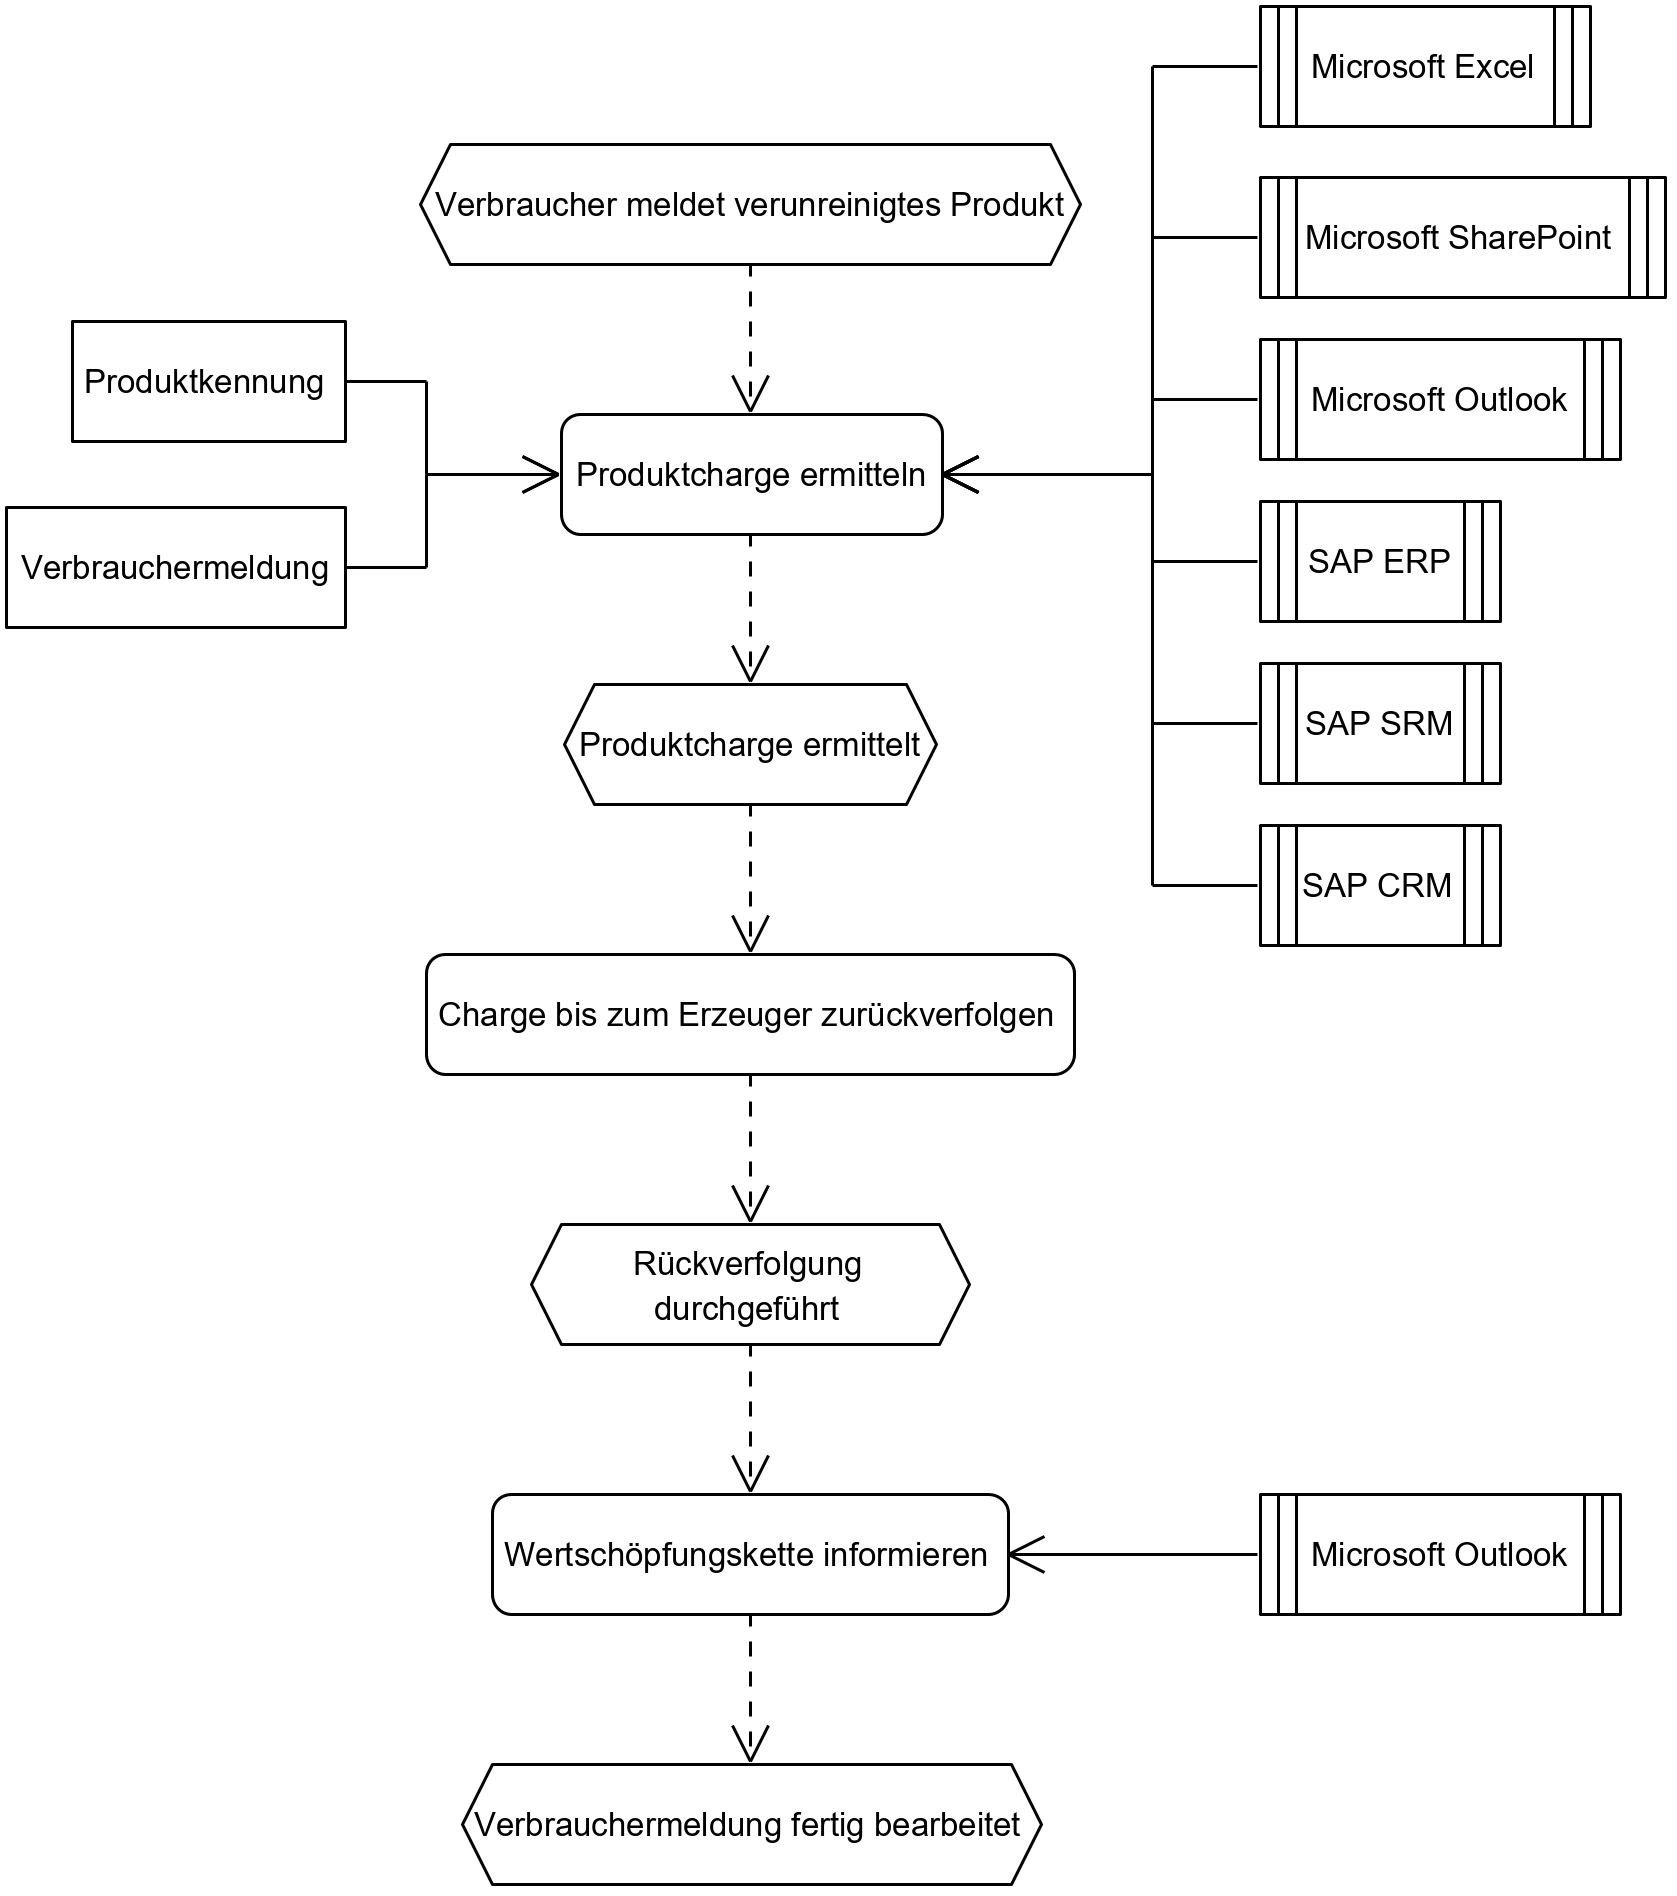
\includegraphics[width=1\linewidth]{pictures/business-process-epc-diagram-bw}
	\caption[Darstellung des Geschäftsprozess Chargenrückverfolgung in eEPK Notation]{Darstellung des Geschäftsprozess Chargenrückverfolgung in eEPK Notation}
	\label{fig:business-process-epc-diagramm}
\end{figure}

\paragraph{Soll-Prozess}
Während im Ist-Prozess (Abbildung \ref{fig:target-business-process}) viele verschiedene IT-Systeme zum Einsatz kommen um alle Chargeninformationen zusammenzutragen, wird im Soll-Prozess das Blockchain Netzwerk und darauf aufsetzende dezentrale Applikationen genutzt. Betrachtet man die einzelnen Prozessschritte so ändert sich bei dem Einsatz einer Blockchain oberflächlich nichts, bei näherer Betrachtung wird dann allerdings deutlich, dass sämtliche Informationen zur Rückverfolgung der Charge vom Blockchain Netzwerk zur Verfügung gestellt werden und nicht in einzelnen Datensilos liegen wie im Ist-Prozess. So dient die Blockchain als gemeinsame Datenbasis für sämtliche Informationen die während der Produktion vom Erzeuger bis zum Lebensmitteleinzelhandel erhoben werden. Änderungen werden transparent in der Blockchain erfasst und sind durch den Konsensmechanismus vor nachträglicher Manipulation geschützt. 

\begin{figure}[H]
	\centering
	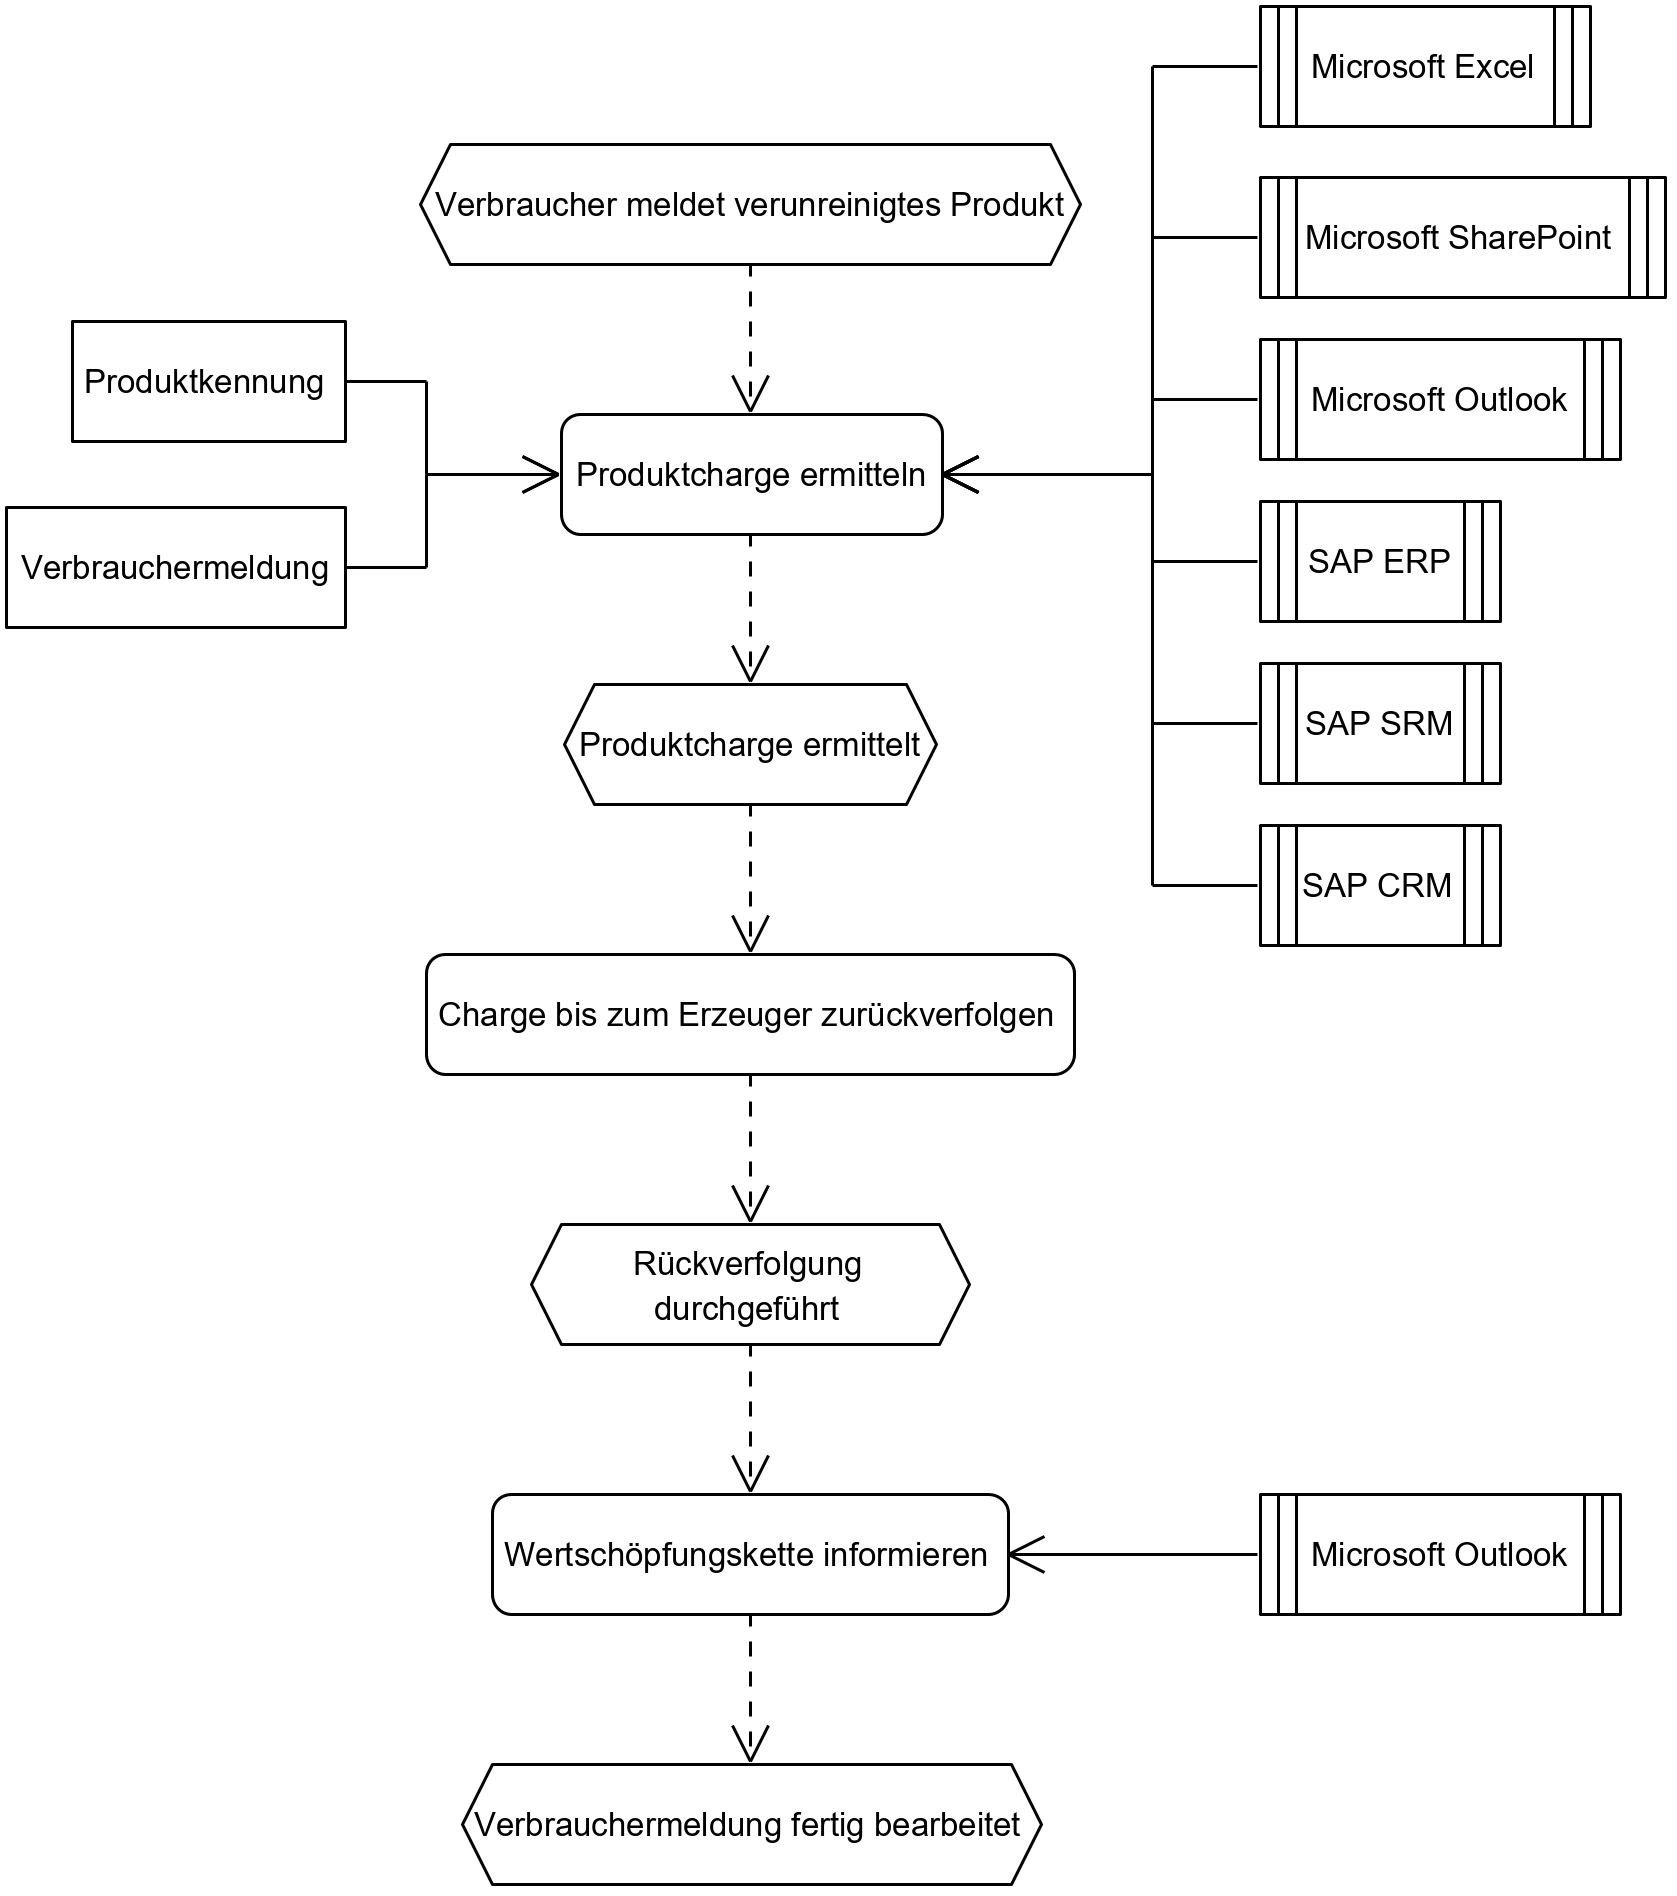
\includegraphics[width=1\linewidth]{pictures/business-process-epc-diagram-bw}
	\caption[Darstellung des Geschäftsprozess Chargenrückverfolgung in eEPK Notation]{Darstellung des Geschäftsprozess Chargenrückverfolgung in eEPK Notation}
	\label{fig:target-business-process}
\end{figure}

\subsection{Funktionale Anforderungen}
1. Alle funktionalen Anforderungen textuell beschreiben und wo sie hergeleitet sind, immer mit Referenz auf die Tabelle in der die Übersicht aller funktionaler Anforderungen zu finden ist.

\begin{table}[H]
    \begin{tabularx}{\textwidth}{@{}lXp{2cm}@{}}
        \toprule
        ID                & Anforderung & Quelle \\
        \midrule
        \textbf{A1.1}              & Das Gesamtsystem muss fähig sein den Lebenszyklus eines Tieres vom Erzeuger bis zum Lebensmitteleinzelhandel abzubilden.                    & \textit{Wissensch. Kontext}                \\ \addlinespace
        \multicolumn{1}{r}{A1.1.1} & Das Gesamtsystem muss fähig sein Tiere anzulegen/registrieren.                     &                 \\ \addlinespace
        \multicolumn{1}{r}{A1.1.2} & Das Gesamtsystem muss fähig sein Tiere und Chargen einander zuzuordnen.                     &                 \\ \addlinespace
        \multicolumn{1}{r}{A1.1.3} & Das Gesamtsystem muss fähig sein Tiere zwischen Teilnehmern zu transferieren im Sinne eines Eigentumswechsel.                     &                 \\
        \textbf{A1.2}              & Das Gesamtsystem muss eine generische Schnittstelle zur Kommunikation mit dem Ledger anbieten.                     & \textit{Partner}                \\ \addlinespace
        \textbf{A1.3}              & Das Gesamtsystem muss fähig sein Transaktionsdaten manipulationssicher speichern zu können.                     & \textit{Partner}                \\ \addlinespace
        \textbf{A1.4}              & Das Gesamtsystem muss fähig sein den Lebenszyklus einer Charge abzubilden.                     & \textit{Partner}                \\ \addlinespace
        \multicolumn{1}{r}{A1.4.1} & Das Gesamtsystem muss fähig sein Chargen anzulegen.                     &                 \\ \addlinespace
        \multicolumn{1}{r}{A1.4.2} & Das Gesamtsystem muss fähig sein Chargen und Tiere einander zuzuordnen.                     &                 \\ \addlinespace
        \bottomrule
    \end{tabularx}
    \caption{Funktionale Anforderungen}
    \label{tab:functional-requirements}
\end{table}

\subsection{Rahmenbedingungen}
1. Alle Rahmenbedingungen textuell beschreiben und wo sie hergeleitet sind, immer mit Referenz auf die Tabelle in der die Übersicht aller Rahmenbedingungen zu finden ist.

\begin{table}[H]
    \begin{tabularx}{\textwidth}{@{}lXp{2cm}@{}}
        \toprule
        ID                & Anforderung & Quelle \\
        \midrule
        \textbf{A2.1}              & Der Prototyp muss mit der Hyperledger Fabric Blockchain Technologie konzipiert und implementiert werden.                     & \textit{Partner}                \\ \addlinespace
        \textbf{A2.2}              & Der Prototyp bildet die Teilnehmer der Wirtschöpfungskette vom Erzeuger bis zum Lebensmitteleinzelhandel ab.                     & \textit{Partner}                \\ \addlinespace
        \textbf{A2.3}              & Der Prototyp fokussiert sich bei der Transaktionsabwicklung auf die Tierart Schwein. (Verminderte Komplexität)                     & \textit{Partner}                \\ \addlinespace
        \bottomrule
    \end{tabularx}
    \caption{Funktionale Anforderungen}
    \label{tab:functional-requirements}
\end{table}

\subsection{Qualitätsanforderungen}
1. Alle Qualitätsanforderungen textuell beschreiben und wo sie hergeleitet sind, immer mit Referenz auf die Tabelle in der die Übersicht aller Qualitätsanforderungen zu finden ist.

\begin{table}[H]
    \begin{tabularx}{\textwidth}{@{}lXp{2cm}@{}}
        \toprule
        ID                & Anforderung & Quelle \\
        \midrule
        \textbf{A3.1}              & Die Architektur des Systems muss eine nachträgliche Erweiterung ermöglichen, um weitere Geschäftszweige abbilden zu können.                     & \textit{Wissensch. Kontext}                \\ \addlinespace
        \textbf{A3.2}              & Die Architektur des Systems muss mindestens eine konstante Performance bei steigender Teilnehmerzahl.                     & \textit{Partner}                \\ \addlinespace
        \textbf{A3.3}              & Das System muss auch bei Ausfall oder Komprimitierung eines oder mehrerer Teilnehmer konsistent und stabil weiter arbeiten.                    & \textit{Partner}                \\ \addlinespace
        \bottomrule
    \end{tabularx}
    \caption{Funktionale Anforderungen}
    \label{tab:functional-requirements}
\end{table}

\subsection{Systementwurf gemäß Architekturkonzept}
Unter berücksichtigung der Resultate aus Kapitel \ref{solution-concept} im Kontext des Anwendungsfalls ergibt sich die Grobarchitektur für das System wie in Abbildung \ref{fig:high-level-architecture} dargestellt.

\begin{figure}[H]
	\centering
	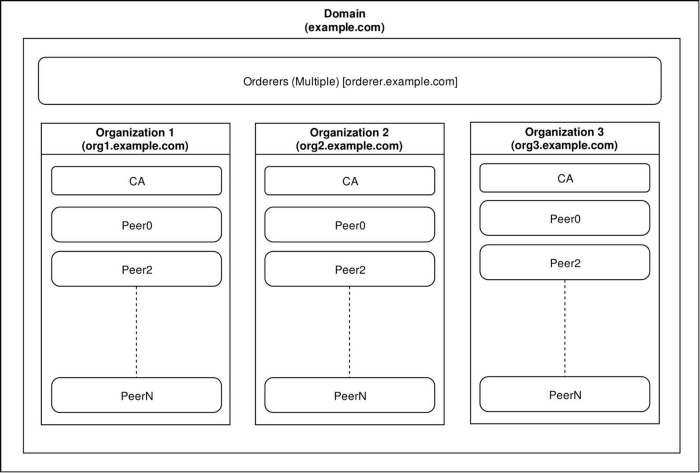
\includegraphics[width=1\linewidth]{pictures/hyperledger-fabric-architecture}
	\caption[High Level System Architecture]{High Level System Architecture}
	\label{fig:high-level-architecture}
\end{figure}

Danach besteht das Gesamtsystem aus logischer Sicht aus dem \textit{Ledger}, einer \textit{Zustandsdatenbank}, den \textit{Smart Contracts} (Chaincode), dem \textit{Konsensmechanismus}, den einzelnen \textit{Teilnehmern} und dem \textit{User Interface}. \textit{Ledger}, \textit{Zustandsdatenbank} und \textit{Smart Contracts} werden zusammen als \textit{Peer} bezeichnet. Zusätzlich gibt es noch eine Sicherheitsstrategie (\textit{CA}) zum Schutz der einzelnen Komponenten. Jeder Teilnehmer des Systems muss mindestens einen \textit{Peer} betreiben, um Transaktionen im Netzwerk erstellen und validieren zu können. Nachfolgend werden die einzelnen Komponenten beschrieben.

\subsubsection{Ledger/Konsens}
Aufbau Ledger (Chain + CouchDB)\\
Transaction Flow mit pBFT\\
1.1 Ledger\\
1.2 Channels\\
1.3 Smart Contracts\\
1.4.4 Endorsement Policies\\
1.4.5 Gossip Protocol\\
2.1 CA\\
2.2 Peers\\
2.2.1 Endorser\\
2.2.2 Anchor\\
2.2.3 General\\
2.3 Orderer\\
5 Transaction Flow\\
5.1 Endorsement\\
5.2 Ordering\\
5.3 Validation

\begin{figure}[H]
	\centering
	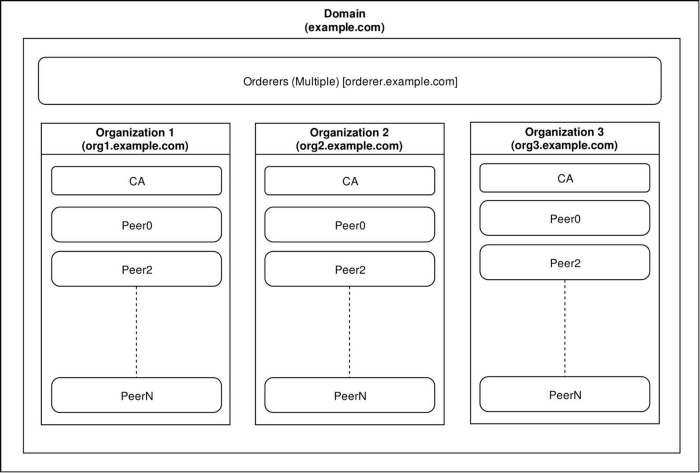
\includegraphics[width=1\linewidth]{pictures/hyperledger-fabric-architecture}
	\caption[Hyperledger Fabric Architecture]{Hyperledger Fabric Architecture (eigene Darstellung)}
	\label{fig:hyperledger-fabric-architecture}
\end{figure}

\begin{figure}[H]
	\centering
	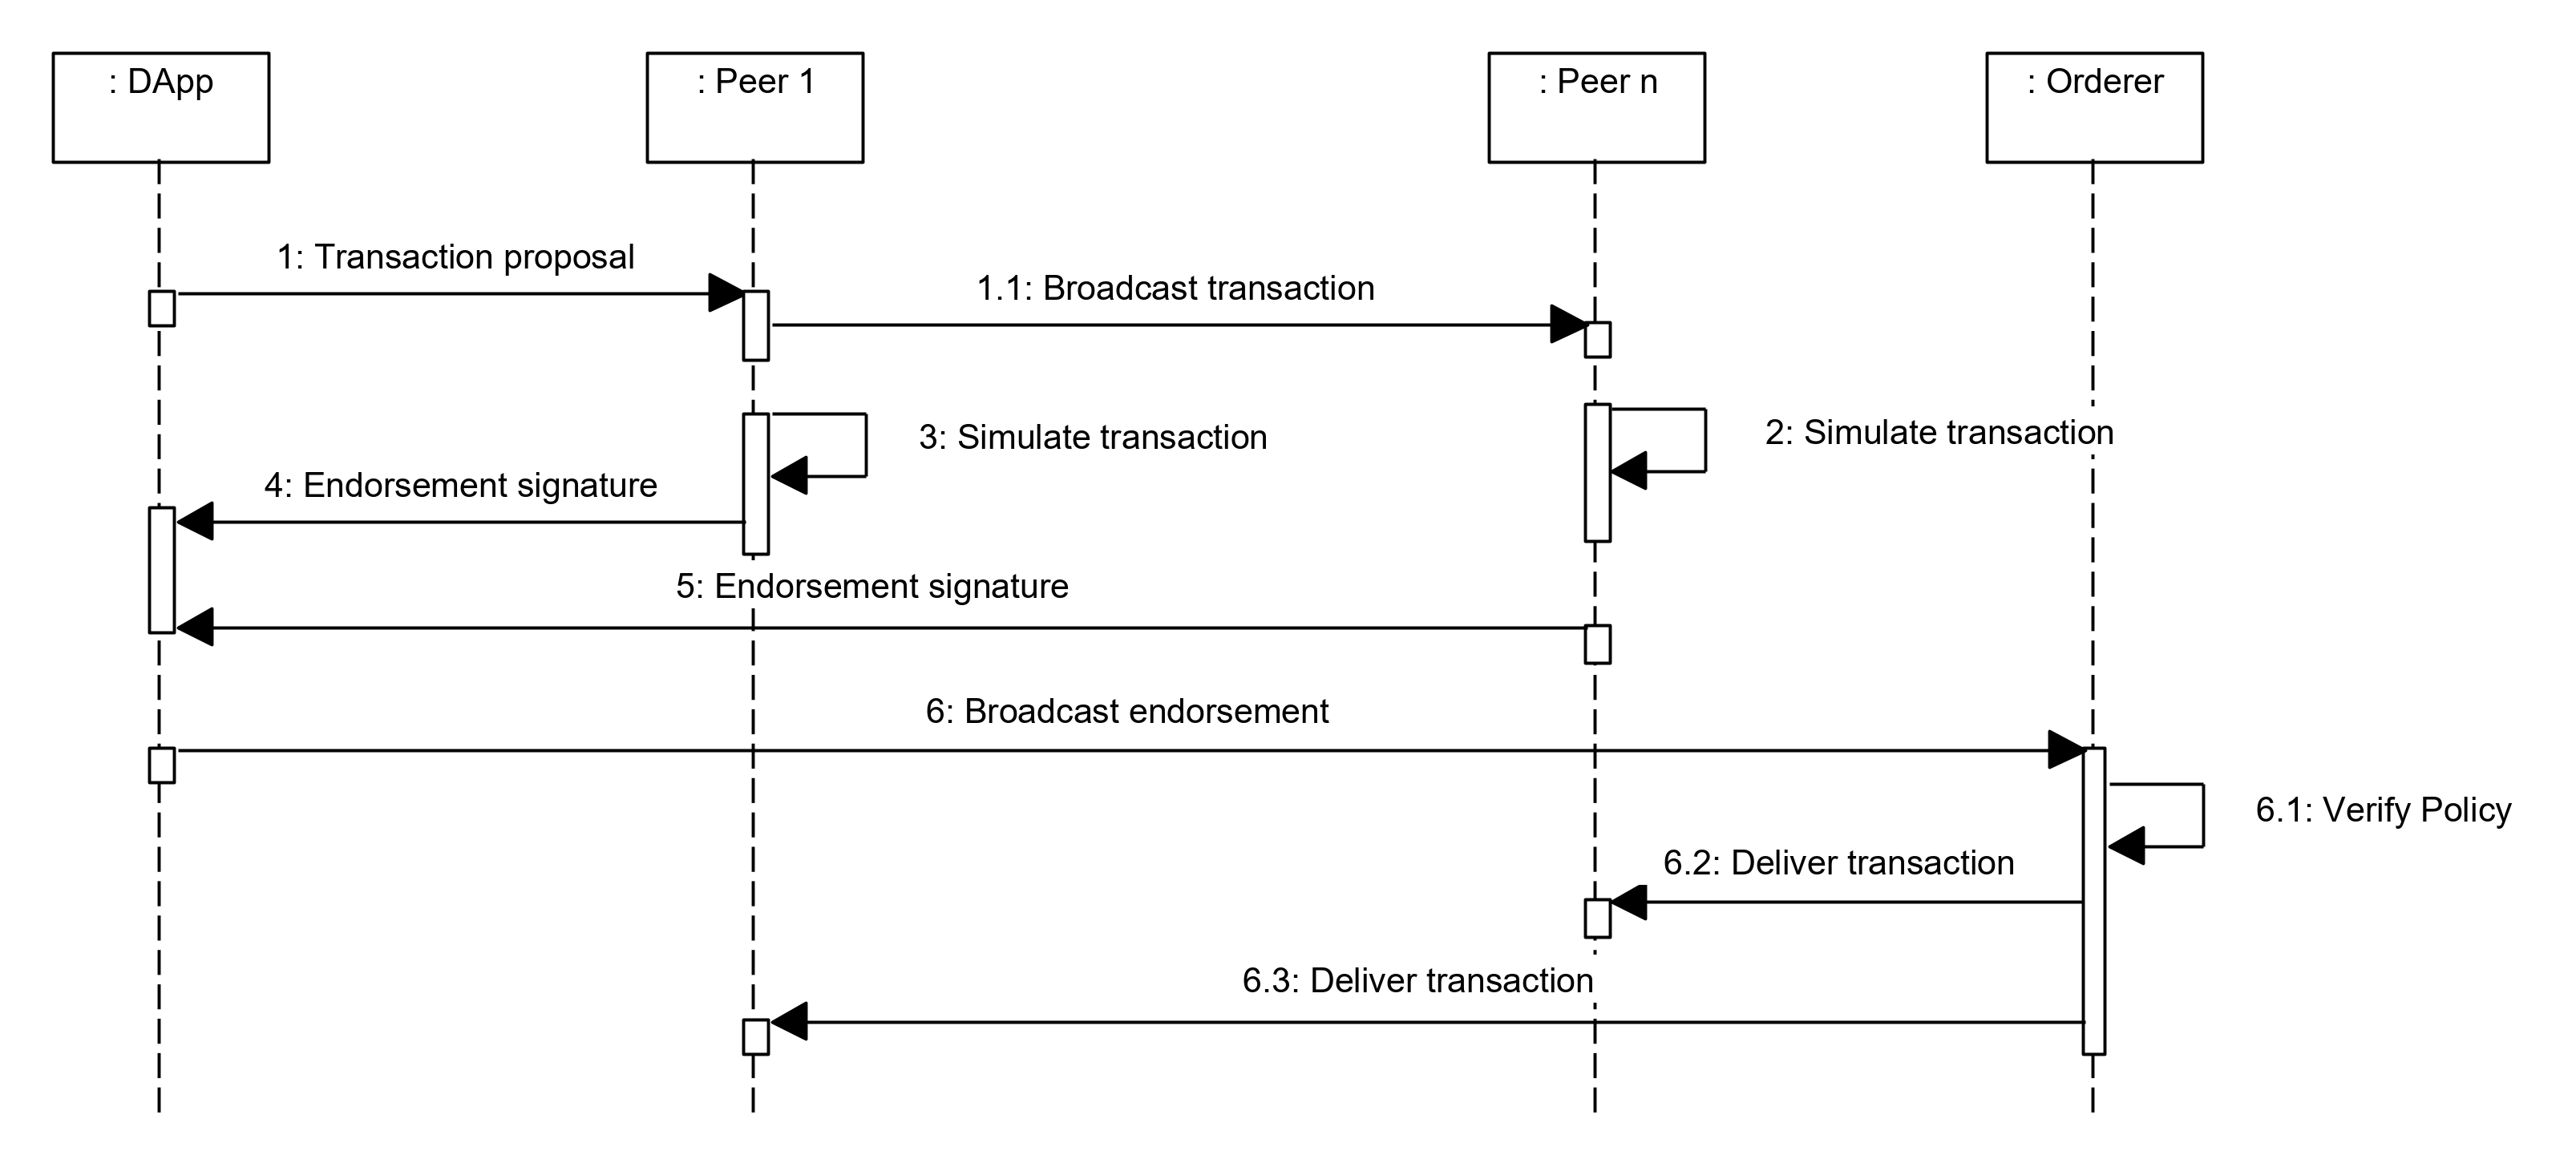
\includegraphics[width=1\linewidth]{pictures/transaction-flow}
	\caption[Transaction Flow]{Transaction Flow in Anlehnung an \citep{Choudhury2018}}
	\label{fig:transaction-flow}
\end{figure}

\subsubsection{Smart Contracts / Business Netzwerk Modell}
Klassendiagramm für Smart Contracts(Transaction Processors), Participants, Assets\\
1.4.2 Assets\\
1.4.3 Transactions\\
1.4.4 Participants

\subsubsection{Identity Management}
PKI\\
1.4.1 Organizations

\subsubsection{API (REST)}
Endpoint Beschreibung\\
3.1 REST API

\subsubsection{User Interface / \DH Apps}
Mockups

\subsubsection{Security / Permissions / Access-Control-List}
Permissions.acl Vorgaben\\
4.1 MSP

\subsection{Zusammenfassung Systementwurf}
1. Anforderungsschema wurde beschrieben\\
2. Ziele wurden erläutert\\
3. Wertschöpfungskette und Geschäftsprozesse wurden dargestellt\\
4. Rahmenbedingungen und Qualitätsanforderungen wurden beschrieben\\
5. Funktionale Anforderungen wurden festgehalten\\
6. Systementwurf wurde dokumentiert\\
7. Ausblick nächstes Kapitel auf konkrete technische Umsetzung

\newpage
